\documentclass[11pt,a4paper]{article}
\usepackage[margin=0.75in]{geometry}
\usepackage[table]{xcolor}
\usepackage{tabularx, multirow, multicol, graphicx, helvet, siunitx, tikz, pgfplots}
\usepackage[most]{tcolorbox}
\renewcommand{\familydefault}{\sfdefault}

%--- colour palette -------------------------------------------------
\definecolor{CorpBlue}{HTML}{003366}
\definecolor{CorpLightBlue}{HTML}{E6F0FA}
\definecolor{CorpGrey}{HTML}{F4F4F4}
\definecolor{AccentRed}{HTML}{CC0000}

%--- pgfplots settings -----------------------------------------------
\pgfplotsset{
    compat=1.18,
    every axis/.append style={
        grid=both,
        grid style={dashed,gray!30},
        axis line style={thick,CorpBlue},
        tick label style={font=\small},
        label style={font=\small}
    }
}

\begin{document}

%=== CORPORATE HEADER =================================================
\noindent
\begin{tabular}{|p{0.32\linewidth}|p{0.34\linewidth}|p{0.30\linewidth}|}
\hline
\textbf{Group:} Materials \& Metallurgy Group &
\textbf{Document Title:} Material Specification &
\textbf{Doc No.:} CRM/MS/01 \\[2mm]
\hline
\textbf{Specification:} 817M40 (EN24) &
\textbf{Sheet:} Sheet &
\textbf{Page:} 1 of 3 \\[2mm]
\hline
\end{tabular}

\vspace{1.5em}

%=== SCOPE / SUMMARY ==================================================
\begin{tcolorbox}[colback=CorpLightBlue,colframe=CorpBlue,
                  title=Scope,
                  fonttitle=\bfseries\large,
                  left=2mm,right=2mm,top=2mm,bottom=2mm]
This document specifies the chemical composition, mechanical properties,
heat‑treatment, surface condition and inspection criteria for the
material 817M40 (EN24) as supplied by the Materials \& Metallurgy Group.
All relevant standards and equivalent specifications are listed herein.
\end{tcolorbox}

%=== CHEMICAL COMPOSITION TABLE =======================================
\vspace{1.5em}
\noindent\textcolor{CorpBlue}{\textbf{\large 1. Chemical Composition}}\vspace{0.5em}

\rowcolors{2}{CorpGrey}{white}
\begin{tabularx}{\linewidth}{|l|c|c|}
\hline
\rowcolor{CorpBlue}\textcolor{white}{\textbf{Element}} &
\textcolor{white}{\textbf{Min (\%)}} &
\textcolor{white}{\textbf{Max (\%)}} \\ \hline
C   & 0.36 & 0.44 \\ \hline
Si  & 0.10 & 0.35 \\ \hline
Mn  & 0.45 & 0.70 \\ \hline
P   & –    & 0.035 \\ \hline
S   & –    & 0.035 \\ \hline
Cr  & –    & 1.40 \\ \hline
Ni  & 1.30 & 1.70 \\ \hline
Mo  & 0.20 & 0.35 \\ \hline
Others & – & – \\ \hline
\end{tabularx}

%=== HARDNESS RANGE GRAPH ============================================
\vspace{1.5em}
\noindent\textcolor{CorpBlue}{\textbf{\large 2. Hardness Requirement}}\vspace{0.5em}

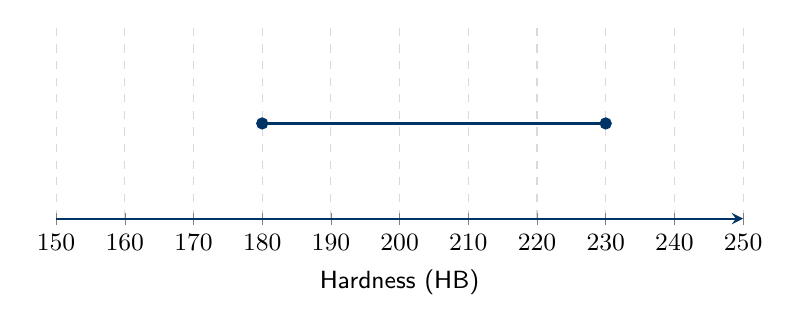
\begin{tikzpicture}
\begin{axis}[
    width=0.85\linewidth,
    height=4cm,
    xlabel={Hardness (HB)},
    ymin=0, ymax=1,
    ytick=\empty,
    xmin=150, xmax=250,
    axis y line=none,
    axis x line=bottom,
    clip=false,
]
\addplot[thick, CorpBlue] coordinates {(180,0.5) (230,0.5)};
\addplot[only marks, mark=*, mark size=2pt, CorpBlue] coordinates {(180,0.5) (230,0.5)};
\end{axis}
\end{tikzpicture}

%=== EQUIVALENT SPECIFICATIONS =======================================
\vspace{1.5em}
\noindent\textcolor{CorpBlue}{\textbf{\large 3. Equivalent Specifications}}\vspace{0.5em}

\rowcolors{2}{CorpGrey}{white}
\begin{tabularx}{\linewidth}{|X|}
\hline
\rowcolor{CorpBlue}\textcolor{white}{\textbf{Specification}} \\ \hline
40Ni6Cr4Mo3 \\ \hline
817M40 (EN24) \\ \hline
36CrNiMo4 \\ \hline
SNCM8 \\ \hline
4340 \\ \hline
IS : 11185 \\ \hline
PD 970-2005 \\ \hline
DIN \\ \hline
JIS \\ \hline
AISI \\ \hline
\end{tabularx}

%=== SECTION 5.1 =====================================================
\vspace{1.5em}
\noindent\textcolor{CorpBlue}{\textbf{\large 5.1. Austenite grain size as per IS 2853/ASTM E112}}\vspace{0.5em}

\rowcolors{2}{CorpGrey}{white}
\begin{tabularx}{\linewidth}{|c|}
\hline
\rowcolor{CorpBlue}\textcolor{white}{\textbf{Grain Size Number}} \\ \hline
5 \\ \hline
6 \\ \hline
7 \\ \hline
8 \\ \hline
\end{tabularx}

%=== SECTION 5.2 =====================================================
\vspace{1.5em}
\noindent\textcolor{CorpBlue}{\textbf{\large 5.2. Inclusion Rating AS 4163/ASTM E45}}\vspace{0.5em}

\rowcolors{2}{CorpGrey}{white}
\begin{tabularx}{\linewidth}{|l|c|c|}
\hline
\rowcolor{CorpBlue}\textcolor{white}{\textbf{Series}} &
\textcolor{white}{\textbf{Code}} &
\textcolor{white}{\textbf{Order}} \\ \hline
\multirow{4}{*}{Thin Series} & ЗА & 1 \\ \cline{2-3}
                              & 3В & 2 \\ \cline{2-3}
                              & 3C & 3 \\ \cline{2-3}
                              & 3D & 4 \\ \hline
\multirow{4}{*}{Thick Series} & 2A & 1 \\ \cline{2-3}
                               & 2B & 2 \\ \cline{2-3}
                               & 2C & 3 \\ \cline{2-3}
                               & 2D & 4 \\ \hline
\end{tabularx}

%=== SECTION 5.3 =====================================================
\vspace{1.5em}
\noindent\textcolor{CorpBlue}{\textbf{\large 5.3. Micro structure As per IS ASTM E407}}\vspace{0.5em}
Uniformly Distributed ferrite \& pearlite should be free from harmful bands.
Max. Limit for banding shall be 0.050 mm. In case of doubt, results from
measurement method should be considered as final.

%=== SECTION 5.4 =====================================================
\vspace{1.5em}
\noindent\textcolor{CorpBlue}{\textbf{\large 5.4. Freedom from defects as per IS:11371}}\vspace{0.5em}
Shall be free from internal \& external surface defects when tested by physical
inspection, ultrasonic method \& macro‑etch method. Shall be free from surface
cracks, seams \& laps, harmful porosity, slag, inclusion, harmful dendritic
structure, segregation \& cracks.

%=== SECTION 5.5 =====================================================
\vspace{1.5em}
\noindent\textcolor{CorpBlue}{\textbf{\large 5.5. Depth of decarburization as per IS:6396}}\vspace{0.5em}
Depth of decarburization when measured in accordance with IS:6396 or any other
method shall not exceed the limit given in table 6 to 8 as in IS:11185.

%=== SECTION 5.6 =====================================================
\vspace{1.5em}
\noindent\textcolor{CorpBlue}{\textbf{\large 5.6. Heat treatment condition as supplied}}\vspace{0.5em}
\begin{itemize}
  \item Annealed / Normalized as hot rolled or forged
\end{itemize}

%=== SECTION 5.7 =====================================================
\vspace{1.5em}
\noindent\textcolor{CorpBlue}{\textbf{\large 5.7. Surface condition as supplied}}\vspace{0.5em}
\begin{itemize}
  \item Black
\end{itemize}

%=== SECTION 5.8 =====================================================
\vspace{1.5em}
\noindent\textcolor{CorpBlue}{\textbf{\large 5.8. Test Certificate}}\vspace{0.5em}
Test certificate shall be provided by the supplier for all specified chemical.

\end{document}